\chapter{Objetivos y Temporización}


El objetivo máximo de este proyecto es realizar un análisis detallado de la plataforma Prado2 que pueda servir como una herramienta para facilitar el trabajo a los administradores de la misma, ya que la evidente falta de recursos del CEVUG hace que un análisis de dichas características sea poco menos que imposible.

\bigskip
Dicho objetivo es el conjunto de los siguientes objetivos principales:

\begin{itemize}
  \item \textbf{OBJ-1.} Analizar la usabilidad de Prado2.
  \item \textbf{OBJ-2.} Analizar la accesibilidad de Prado2.
  \item \textbf{OBJ-3.} Analizar la seguridad de Prado2.
  \item \textbf{OBJ-4.} Analizar la disponibilidad de Prado2.
  \item \textbf{OBJ-5.} Promover la idea de que los desarrollos bajo software libre en general y en la administración pública en particular ayudan a generar confianza y demuestran compromiso.
  
\end{itemize}

Además como objetivos secundarios tendremos:

\begin{itemize}
  \item \textbf{OBJ-6.} Estudiar la posibilidad de hacer un clon de la instalación actual de Prado2 en un servidor propio.
  \item \textbf{OBJ-7.} Estudiar la posibilidad de desarrollar una herramienta para solventar los problemas de usabilidad de la plataforma. 
  \item \textbf{OBJ-8.} Estudiar la posibilidad de desarrollar una herramienta para solventar los problemas de seguridad de la plataforma. 
   \item \textbf{OBJ-9.} Estudiar la posibilidad de configurar un dispositivo hardware para analizar la seguridad de la plataforma.
\end{itemize}



\section{Alcance de los objetivos}
El fin inmediato de este informe es servir de herramienta a los administradores de la plataforma para que conozcan los fallos más importantes y sugerencias sobre como solucionarlos.
Además el informe resultante se liberará con una licencia libre para que cualquier parte interesada pueda hacer uso las conclusiones y los datos extraídos del análisis.

\section{Interdependencia de los objetivos}

Todos los objetivos son independientes entre sí, pero el primer objetivo (\textbf{OBJ-1}) es el principal motivador de este proyecto, por lo que aún sin representar el desarrollo de ningún trabajo en concreto es el que va a escudar y avalar el desarrollo de los otros. En aspectos más relacionados con la realización del proyecto, el tercer objetivo (\textbf{OBJ-3}) es el que se requerirá solucionar de forma inmediata, ya que impide el correcto funcionamiento del portal. El resto de objetivos serán tratados en mayor o menor medida.

\section{Conocimientos y herramientas utilizadas}

\bigskip
Destacar en los aspectos formativos previos más utilizados para el desarrollo del proyecto los conocimientos sobre Desarrollo de Aplicaciones para Internet para el análisis de usabilidad y accesibilidad, Fundamentos de Ingeniería de Software para el análisis del proyecto, Seguridad en Sistemas Operativos para la parte de seguridad y Servidores Web de Altas Prestaciones para la realización de pruebas desde el punto de vista de disponibilidad y carga de trabajo.

Para la realización de cada una de las partes se han usado multitud de herramientas específicas tales como pueden ser WireShark, ettercap, statusCake, Latex, R, Google Forms y Google SpreadSheets entre otras. 


\section{Temporización estimada}


En la figura \ref{fig:temporizacion1} podemos ver la planificación de tiempos para el desarrollo de este proyecto. 

\begin{figure}[H]
\centering
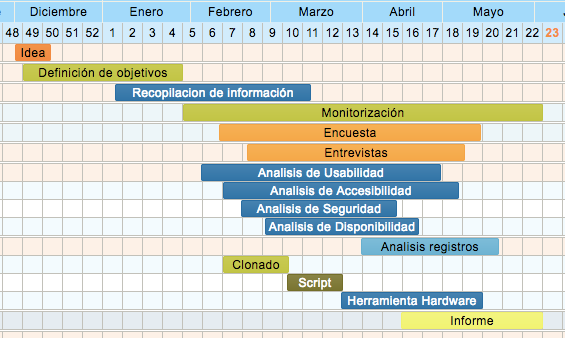
\includegraphics[width=0.8\textwidth]{../screenshots/temporizacion1}
\caption{Diagrama de Gantt con los tiempos estimados para el proyecto}
\label{fig:temporizacion1}
\end{figure}







